\doublespacing % Do not change - required

\chapter{Introduction}
\label{ch1}

%%%%%%%%%%%%%%%%%%%%%%%%%%%%%%%%%%%%%%%
% IMPORTANT
\begin{spacing}{1} %THESE FOUR
\minitoc % LINES MUST APPEAR IN
\end{spacing} % EVERY
\thesisspacing % CHAPTER
% COPY THEM IN ANY NEW CHAPTER
%%%%%%%%%%%%%%%%%%%%%%%%%%%%%%%%%%%%%%%


\section{Title section}

\kant[1]

Example of citation are here
\cite{AdaAroKre:71,PadScaAst:16a,PadScaAst:16b,PavVdWNij:06,PurBorVar:96,SLICOT,Sca:16,Sca:16a,Sca:16b,Sca:17,Sca:18}.

And some acronyms: \ac{USA} and \ac{LTI} systems.

\subsection{Title subsection}

\kant[1-10]


\begin{figure}
\centering
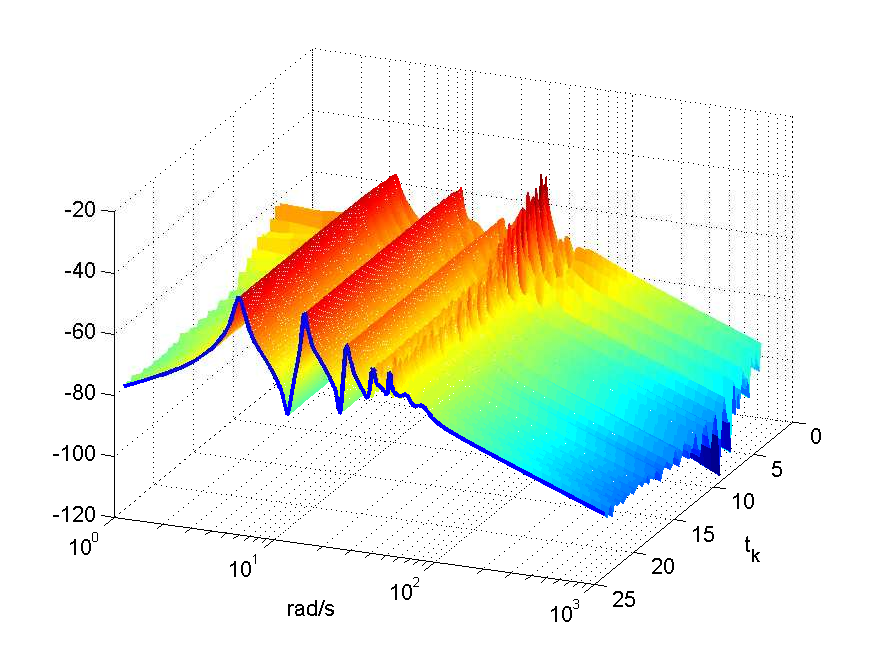
\includegraphics[width=0.8\columnwidth]{imgs/buildmagnitude.pdf}
\caption[Short description for list of figures]{This figure is taken from \cite{Sca:16}.}
\label{fig-magnitude}
\end{figure}%


\kant[1-4]

\subsection{Title subsection}

\kant[1-3]


\section{Title section}

\kant[1-5]

\section{Notation}

Standard notation has been adopted in the Thesis, most of which is defined in this section and used throughout the remainder of the Thesis. When new notation, not included in this section is introduced, this is defined in the relevant parts of the Thesis.\smallskip\\
\indent The symbol $\mathbb{R}_{\ge0}$ ($\mathbb{R}_{>0}$) denotes the set of non-negative (positive) real numbers; $\mathbb{C}_{<0}$ denotes the set of complex numbers with strictly negative real part; $\mathbb{C}_{0}$ denotes the set of complex numbers with zero real part and $\mathbb{D}_{<1}$ the set of complex numbers with modulo less than one.\smallskip\\
\indent The symbol $I$ denotes the identity matrix and $\sigma(A)$ denotes the spectrum of the matrix $A\in\mathbb{R}^{n\times n}$. The symbol $\otimes$ indicates the Kronecker product and $||A||$ indicates the induced Euclidean matrix norm. Given a list of $n$ elements $a_i$, $\diag(a_i)$ indicates a diagonal matrix with diagonal elements equal to the $a_i$'s. The vectorization of a matrix $A\in\mathbb{R}^{n\times m}$, denoted by $\vect(A)$, is the $nm \times 1$ vector obtained by stacking the columns of the matrix $A$ one on top of the other, namely $\vect(A)=[a_1^{\top},a_2^{\top},\dots,a_m^{\top}]^{\top}$, where $a_i\in\mathbb{R}^n$ are the columns of $A$ and the superscript $\top$ denotes the transposition operator. The superscript $*$ indicates the conjugate transpose operator.\smallskip\\
\indent The symbol $\Re[z]$ indicates the real part of the complex number $z$, $\Im[z]$ denotes its imaginary part and $\iota$ denotes the imaginary unit. The symbol $\epsilon_k$ indicates a vector with the $k$-th element equal to 1 and with all the other elements equal to 0. Given a function $f$, $\overline{F}$ represents its phasor at $\omega$, whereas $<\!f(t)\!>$ indicates its time average.\smallskip\\
\indent Given a set of delays $\{\tau_j\}$, the symbol $\mathfrak{R}_T^n=\mathfrak{R}_T^n([-T,0],\mathbb{R}^n)$, with $T=  \max_j\{\tau_j\}$, indicates the set of continuous functions mapping the interval $[-T,0]$ into $\mathbb{R}^n$ with the topology of uniform convergence . The subscripts ``$\tau_j$'' and ``$\chi_j$'' denote the translation operator, \textit{e.g.}\ $x_{\tau_j}(t)=x(t-\tau_j)$.\smallskip\\
\indent Let $\bar s \in \mathbb{C}$ and $A(s)\in \mathbb{C}^{n \times n}$. Then $\bar s\notin\sigma(A(s))$ means that $\det(\bar s I-A(\bar s ))\ne0$. $\sigma(A(s))\subset\mathbb{C}_{<0}$ means that for all $\bar s$ such that $\det(\bar s I-A(\bar s ))=0$, $\bar s \in\mathbb{C}_{<0}$.\smallskip\\
\indent The symbol $\mathcal{L}(f(t))$ denotes the Laplace transform of the function $f(t)$ (provided that $f(t)$ is Laplace transformable) and $\mathcal{L}^{-1}\{F(s)\}$ denotes the inverse Laplace transform of $F(s)$ (provided it exists). With some abuse of notation, $\sigma(\mathcal{L}(f(t)))$ denotes the set of poles of $\mathcal{L}(f(t))$. Given two functions, $f:Y\to Z$ and $g:X\to Y$, with $f\,\circ\,g:X\to Z$ we denote the composite function $(f\,\circ\,g)(x)=f(g(x))$ which maps all $x\in X$ to $f(g(x))\in Z$.


\section{Published material}

\kant[1]
